\part{Test Strategy}

\begin{frame}{Motivation}
	\textbf{Goal:} Ship \emph{any} kind of change \emph{within a day}
	\vfill

	\begin{visibleenv}<2->	
	  \begin{block}{Prerequisite: Automated Tests}
	  \begin{columns}
		\begin{column}{0.7\textwidth}
		\begin{itemize}
		  \item Basis for automated delivery pipeline
		  \item Hinders deployment of unworthy changes
		  \item Keeps you relaxed \ldots
		\end{itemize}
		\end{column}
		\begin{column}{0.25\textwidth}
		  \hspace{-7mm}
		  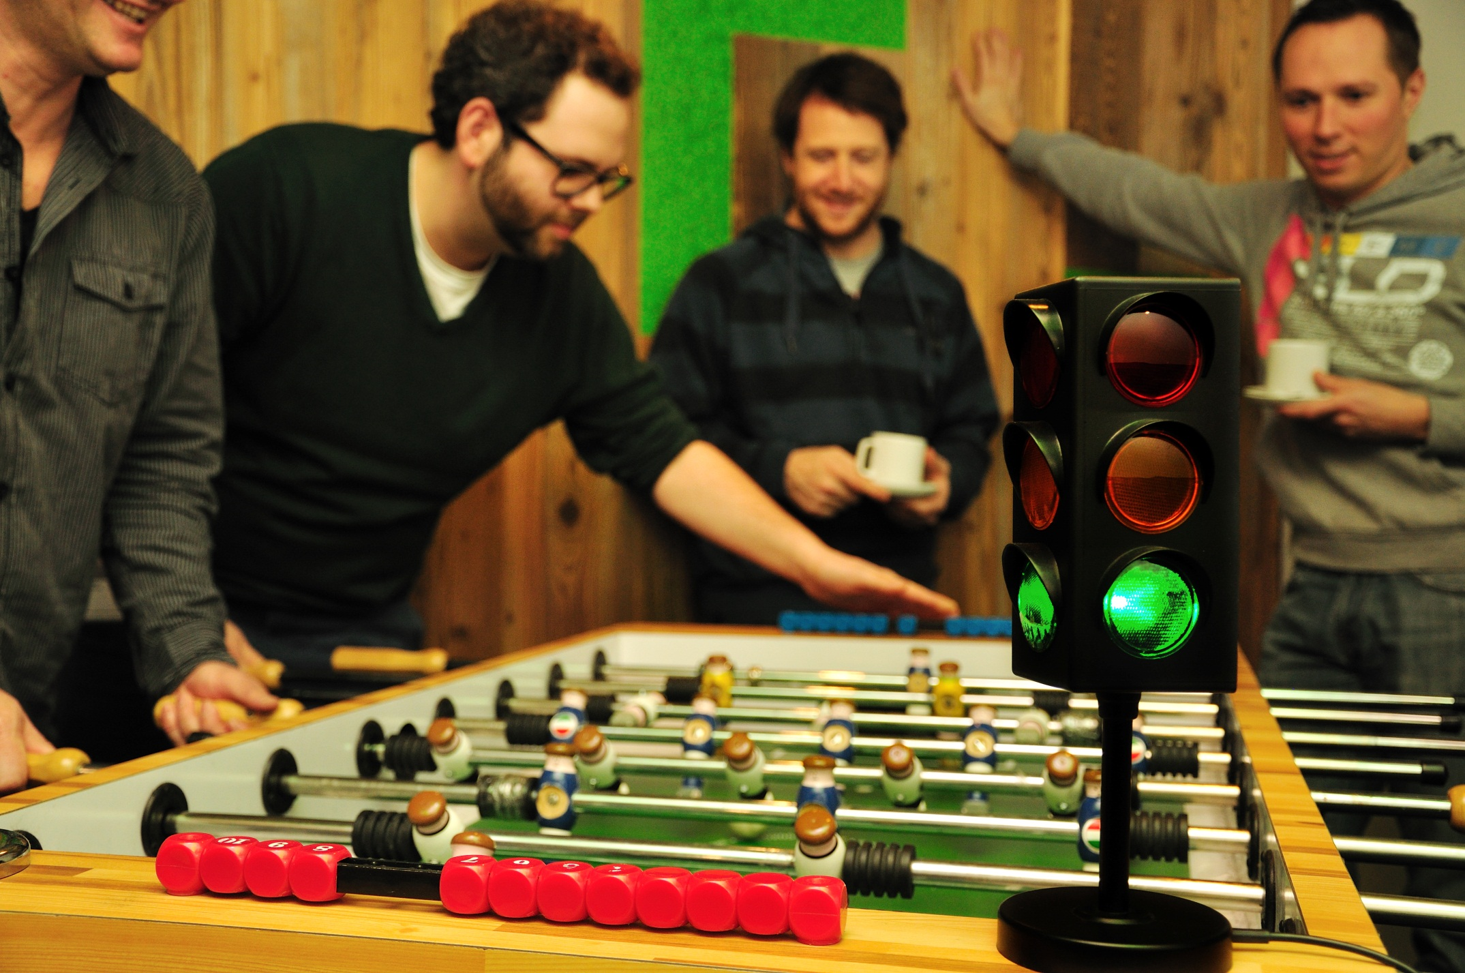
\includegraphics[width=35mm]{../ContinuousDelivery/images/Relaxed_Before_Deployment}\\
		\end{column}
	  \end{columns}
	  \end{block}
	  \end{visibleenv}
	\vfill
	
	\visible<3->{\centerline{\textbf{What is an effective test strategy?}}}
\end{frame}

\begin{frame}{Agile Testing Strategy}
\vspace{5mm}
Implement \colorlink{https://wiki.wdf.sap.corp/wiki/display/ASE/Agile+Test+Automation+Strategy}{Testing Pyramid} to gain solid safety net
\only<1>{
	\begin{figure}
	   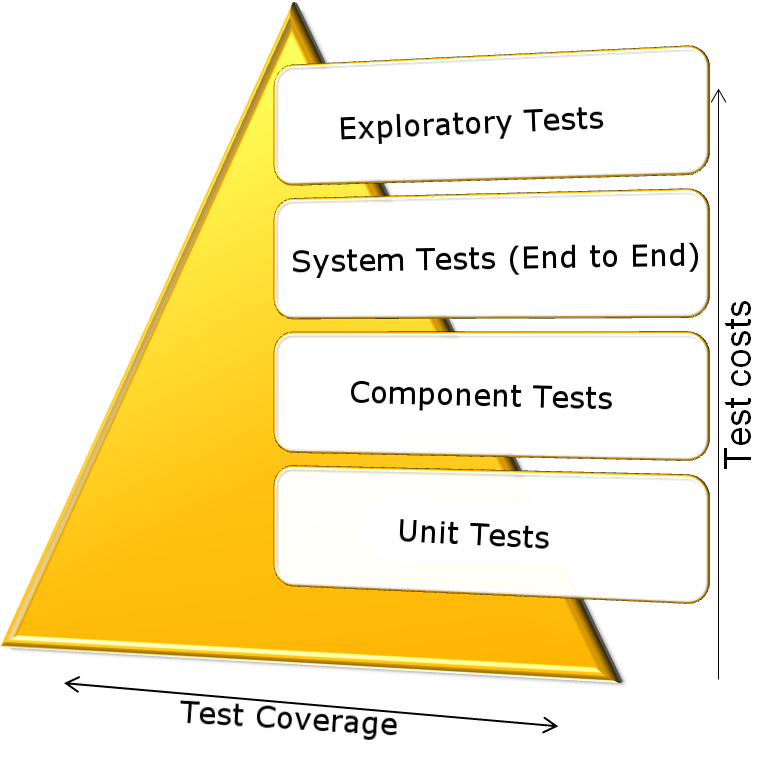
\includegraphics[height=0.6\textheight]{../TestStrategy/images/TestPyramid}
	\end{figure}
}

\visible<2->{
	%\vspace{-5mm}
	\begin{figure}
	 \begin{flushright}
	   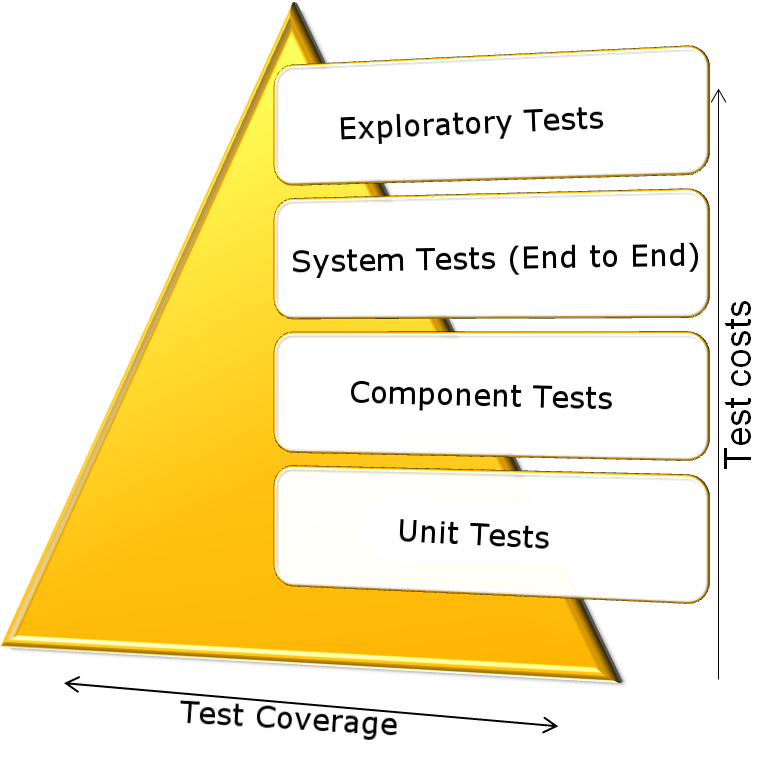
\includegraphics[height=2cm]{../TestStrategy/images/TestPyramid}
	 \end{flushright}
	\end{figure}
	\vspace{-25mm}
	\begin{itemize}
		\item \textbf{Reduce Test Scope}: \\Easier to write and maintain, eases error localization
		\item \textbf{Focus} on testing your \textbf{\emph{own} code and functionality}
		\item Test interaction of services using \textbf{system tests}
		\item Different kinds of tests should \textbf{complement} each other
	\end{itemize}
}
\end{frame}

\begin{frame}{Unit Tests}
\begin{figure}
\includeGraphicsUnitTest{height=0.5\textheight}
\end{figure}
\vfill
\begin{block}{Test business logic in isolation}
\begin{itemize}
	\item Test most combinations and error cases
	\item \colorlink{https://github.com/ccjavadev/cc-bulletinboard-ads-spring-webmvc/blob/solution-9-Implement-JPA-Entity/src/test/java/com/sap/bulletinboard/ads/models/AdvertisementRepositoryTest.java}{Example}: Test valid/invalid cases updating an advertisement 
\end{itemize}
\end{block}
\end{frame}

\begin{frame}{Component Tests}
\begin{figure}
\includeGraphicsComponentTest{height=0.5\textheight}
\end{figure}
\vfill
\begin{block}{Test in runtime environment, without external dependencies}
\begin{itemize}
	\item Tests code integration with libraries and frameworks incl. security
	\item \colorlink{https://github.com/ccjavadev/cc-bulletinboard-ads-spring-webmvc/blob/solution-4-2-DeleteUpdate/src/test/java/com/sap/bulletinboard/ads/controllers/AdvertisementControllerTest.java}{Example:} Update the title of an advertisement via REST-like API
\end{itemize}
\end{block}
\end{frame}

\begin{frame}{System Tests}
\begin{figure}
\includeGraphicsSystemTest{height=0.5\textheight}
\end{figure}
\vfill
\begin{block}{Test combination of services \textit{deployed on Cloud Foundry test space}}
\vspace{-2mm}
\begin{itemize}
	\item Tests integration end to end (\colorlink{http://martinfowler.com/articles/microservice-testing/\#testing-end-to-end-tips}{further tips})
	\\Requires configurable routes to dependent services, and data
	\item \colorlink{https://github.wdf.sap.corp/cc-java/cc-bulletinboard-systemtest/blob/master/src/test/java/com/sap/bulletinboard/systemtests/SystemTest.java}{Example:} 
	Create advertisement via REST, call external user service
\end{itemize}
\vspace{-3mm}
\end{block}
\end{frame}

\begin{frame}{Test Focus}
\begin{center}
	\textbf{Which tests covers these cases?}\\
	(from the perspective of the Advertisement Service)
\end{center}
\begin{center}
\begin{tabular}{lr}
\textbf{Test Case} & \textbf{Test} \\
\hline
Entities are persisted & \visible<2->{\alert<2>{Component}}\\
\visible<3->{Successful connection to the database in the cloud}	& \visible<4->{\alert<4>{System}}\\
\visible<5->{Every advertisement has a non-empty title}			& \visible<6->{\alert<6>{Unit}}\\
\visible<7->{For each timeout a log message is shown}			& \visible<8->{\alert<8>{Unit}}\\
\visible<9->{The REST endpoints are available via HTTP}			& \visible<10->{\alert<10>{Component}}\\
\visible<11->{JSON in User service response contains expected fields}   & \visible<12->{\alert<12>{???}}\\
\end{tabular}
\end{center}
\end{frame}

\begin{frame}{Contract Tests}
\centerline{
		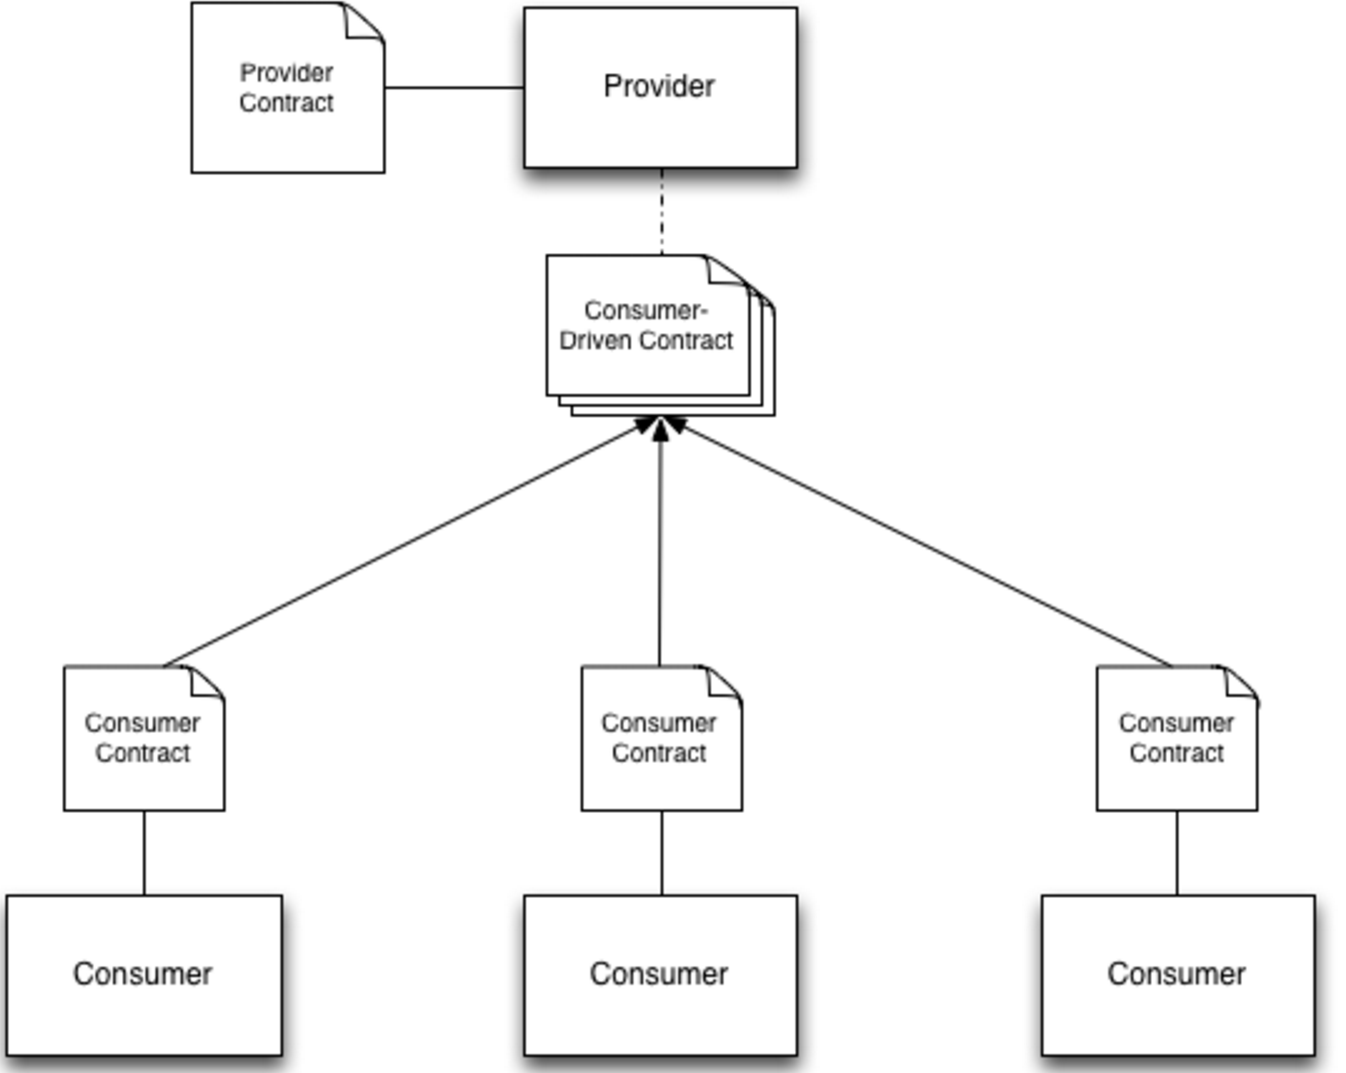
\includegraphics[height=0.47\textheight]{../TestStrategy/images/ConsumerContract}
}
\begin{block}{Test provider's implementation against consumers' requirements}
\vspace{-2mm}
\begin{itemize}
    \item Tests are defined by consumers
    \item Provider considers consumers' tests
    \item Example: self-contained JUnit tests in provider's code base
\end{itemize}
\vspace{-2mm}
\end{block}

\colorlink{https://github.wdf.sap.corp/cc-devops-course/coursematerial/blob/master/ContinuousDelivery/Testing_Version_Combinations/Testing_Version_Combinations.md}{The Dilemma of Testing Microservices in Integration}
\end{frame}

% https://jaxenter.de/microservices-consumer-driven-contract-testing-mit-pact-20574

\begin{frame}{Excursion: \codealt{Muenchhausen} as Fake Identity Provider} 
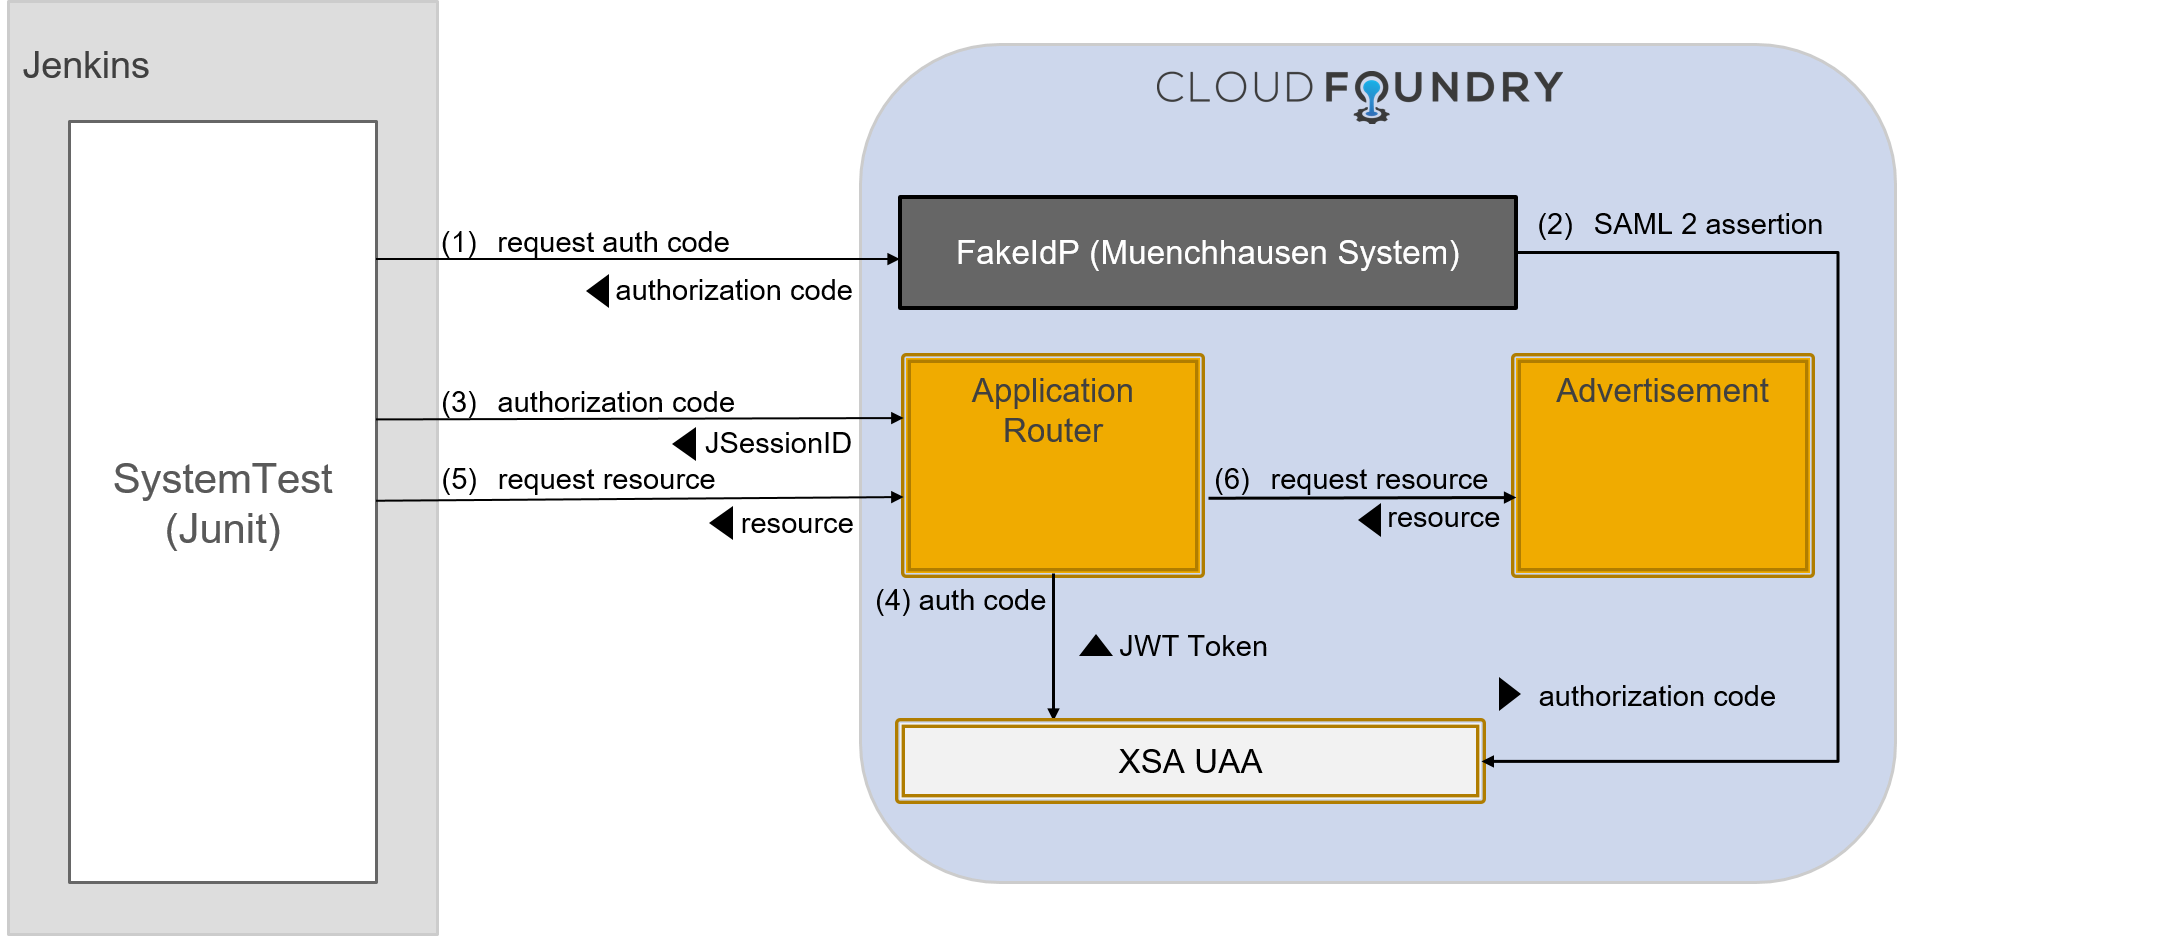
\includegraphics[height=0.65\textheight]{../TestStrategy/images/SystemTest_detailed}
\small
\\\colorlink{https://xsuaa-monitoring-idp.cfapps.sap.hana.ondemand.com/}{\codealt{Muenchhausen}}
\begin{itemize}
    \item Creates SAML2 assertion for fake user with specified SAML2 user groups
    %\item Has a trusted realtionship with the XS UAA
\end{itemize}
\end{frame}

\begin{frame}{Exercise 25}
	\begin{figure}
		\includeGraphicsExerciseTwentyFive{width=1.0\textwidth}
	\end{figure}
	\vfill
	\colorlink{https://github.com/ccjavadev/cc-coursematerial/blob/master/TestStrategy/Exercise_25_Create_SystemTest.md}{Exercise 25: Create and Configure System Test using \codealt{Muenchhausen}}
\end{frame}

\begin{frame}[fragile]{Performance Tests}{Find performance drops or bottlenecks before production}
	\begin{figure}
	\includeGraphicsPerformanceTest{height=0.5\textheight}
	\end{figure}
	\vfill
	\begin{block}{Test expected load (\# concurrent users, \# HTTP connections)}
	\vspace{-2mm}
	\begin{itemize}
		\item Tests whether response time is below threshold 
		\item \colorlink{https://github.com/ccjavadev/cc-coursematerial/blob/master/TestStrategy/JMeterPerformanceTestPlan_security.jmx}{Example}: Create, read many ads in parallel via multi-tenant approuter and Muenchhausen. 
	\end{itemize}
	\end{block}
\end{frame}

\begin{frame}[fragile]{JMeter Demo}
	\centerline{
		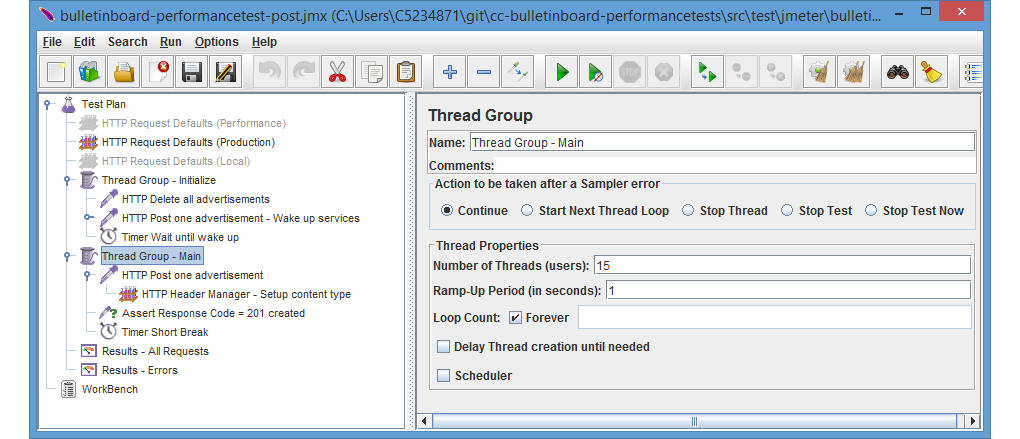
\includegraphics[height=30mm]{../TestStrategy/images/JMeter}
	}
	\begin{itemize}
		\item Scriptable
		\item Master-Slave support
		\item Expandable through plugins
		\item Plugins for Maven and Jenkins
		%\item Alternatives \colorlink{http://locust.io}{locust.io}, \colorlink{http://gatling.io}{gatling.io}, \colorlink{http://grinder.sourceforge.net/}{The Grinder}
	\end{itemize}
	\vfill
	\colorlink{https://github.com/ccjavadev/cc-coursematerial/blob/master/TestStrategy/Exercise_26_PerformanceTesting_With_JMeter.md}{Exercise: Performance testing with JMeter}
\end{frame}

\begin{frame}[fragile]{Performance Testing Remarks}
	\begin{itemize}
		\item Performance tests prone to fluctuations, especially in the cloud
		\item Resilience libraries influence test results (Hystrix) 
		\item Averages or percentiles are misleading, measure maximum instead!
			\begin{itemize}		
				\item Many requests per page => worst case performance is relevant 
			\end{itemize}
		\item In addition make use of performance monitoring
		\begin{itemize}		
			\item Example: Measure latency for downstream requests
		\end{itemize}	
	\end{itemize}
\end{frame}

\begin{frame}{Take Aways}
\begin{itemize}
	\item Write tests according to the Test Pyramid\\
	e.g. write as few end-to-end tests as possible (\colorlink{http://martinfowler.com/articles/microservice-testing/\#testing-end-to-end-tips}{Reference}) 
	\item Write black box tests (test visible behavior of public methods)
	\item Practice Test Driven Development (TDD)
	\item Execute tests locally before submitting changes
	\item Setup local/test environment similar to production
\end{itemize}
Note: You are unable to test each and everything!

\vspace{1cm}

\centerline{\textbf{In addition to testing: extensive monitoring}}
\end{frame}
